\documentclass[9pt]{pnas-new}
% Use the lineno option to display guide line numbers if required.
% Note that the use of elements such as single-column equations
% may affect the guide line number alignment. 

%\RequirePackage[english,slovene]{babel} % when writing in slovene
%\RequirePackage[slovene,english]{babel} % when writing in english

\templatetype{pnasresearcharticle} % Choose template 
% {pnasresearcharticle} = Template for a two-column research article
% {pnasmathematics} = Template for a one-column mathematics article
% {pnasinvited} = Template for a PNAS invited submission

%\selectlanguage{slovene}
%\etal{in sod.} % comment out when writing in english
%\renewcommand{\Authands}{ in } % comment out when writing in english
%\renewcommand{\Authand}{ in } % comment out when writing in english

\newcommand{\set}[1]{\ensuremath{\mathbf{#1}}}
\renewcommand{\vec}[1]{\ensuremath{\mathbf{#1}}}
\newcommand{\uvec}[1]{\ensuremath{\hat{\vec{#1}}}}
\newcommand{\const}[1]{{\ensuremath{\kappa_\mathrm{#1}}}} 

\newcommand{\num}[1]{#1}

\graphicspath{{./fig/}}

\title{Nest-site selection in mass-recruiting ant species}

% Use letters for affiliations, numbers to show equal authorship (if applicable) and to indicate the corresponding author
\author{Meggy-Lie-Anne Chamand}
\author{Kim Georget}
\author{Bella Muradian}
\author{Clara Stavun}

\affil{Collective behaviour course research seminar report} 

% Please give the surname of the lead author for the running footer
\leadauthor{Chamand} 

\selectlanguage{english}


% Please add here a significance statement to explain the relevance of your work
\significancestatement{Programmable modeling environment}{To solve the problem written above, we will use an agent-based model built in NetLogo. NetLogo is a widely used, user-friendly agent-based modeling environment tailored for simulating complex systems, making it ideal for studying ant social behavior and collective decision-making with its visual interface and real-time simulations.

It's worth noting that the NetLogo platform, while effective for simulating ant behavior, has limitations, especially in terms of visual representation. We could only use basic shapes (circles, triangles, stars) in limited colors to represent our elements (food, predators, protection). 
}

\selectlanguage{english}

% Please include corresponding author, author contribution and author declaration information
%\authorcontributions{Please provide details of author contributions here.}
%\authordeclaration{Please declare any conflict of interest here.}
%\equalauthors{\textsuperscript{1}A.O.(Author One) and A.T. (Author Two) contributed equally to this work (remove if not applicable).}
%\correspondingauthor{\textsuperscript{2}To whom correspondence should be addressed. E-mail: author.two\@email.com}

% Keywords are not mandatory, but authors are strongly encouraged to provide them. If provided, please include two to five keywords, separated by the pipe symbol, e.g:
\keywords{Agent-based model | New nest-site choice | Mass-recruiting ant | Quorum | simulation} 

\begin{abstract}
This study explores the intricate behavior of ant colonies, focusing on the nest emigration process of the M. nipponica ant. Utilizing an agent-based model in NetLogo, we investigate the collective decision-making of ants during nest selection. We focus on finding the best possible nest and we introduce new parameters, such as food, protection, and predators near nests, influencing nest quality. The model distinguishes four ant types and dynamically adjusts their threshold for labeling nests as 'good' or 'bad.' Through simulations, we assess the impact of parameters like quorum percent, commitment base, and pheromone deposition on nest selection.
\end{abstract}

\dates{\textbf{\today}}
\program{BM-RI}
\vol{2018/19}
\no{CB:GH} % group ID
%\fraca{FRIteza/201516.130}

\begin{document}

% Optional adjustment to line up main text (after abstract) of first page with line numbers, when using both lineno and twocolumn options.
% You should only change this length when you've finalised the article contents.
\verticaladjustment{-2pt}

\maketitle
\thispagestyle{firststyle}
\ifthenelse{\boolean{shortarticle}}{\ifthenelse{\boolean{singlecolumn}}{\abscontentformatted}{\abscontent}}{}

% If your first paragraph (i.e. with the \dropcap) contains a list environment (quote, quotation, theorem, definition, enumerate, itemize...), the line after the list may have some extra indentation. If this is the case, add \parshape=0 to the end of the list environment.
\dropcap{S}ocial insects have simple yet captivating individuals and thus provide an ideal subject for scientific exploration. This study delves into the intricate behavior of ant colonies, particularly during the emigration process to new nests, with a specific focus on the nest emigration process of the M. nipponica ant. Our research aims to unravel the complexities of ant colony behavior in the context of new nest selection, by examining various parameters, including the quorum percent, commitment base, and pheromone deposition, to understand their collective role in decision-making.

While significant strides have been made in understanding ant colonies, certain aspects, such as behavioral rules, remain elusive. Simultaneously, existing models contribute to giving valuable insights into how ants collectively decide on nest-site selection. For instance, mass-recruiting algorithms emulate complex collective biological processes \cite{computational_model}, while quorum-sensing mechanisms rely on cumulative pheromone thresholds for nest-site selection \cite{quorum_sensing_recruitment}. Additionally, models consider variable acceptance thresholds, reflecting diverse ant preferences, and individual assessment behavior, where some ants prioritize proximity to food sources, while others favor concealment from predators \cite{variability_individual_assessment}.

However, existing models often focus on specific parameters, hindering a comprehensive assessment of their relative influence. In response, our research adopts a holistic approach, integrating multiple parameters to elucidate their collective impact on decision-making processes during nest emigration. The paper we selected aimed to contribute to a more nuanced understanding of the intricate dynamics within ant colonies during new nest selection, by trying to determine how ants choose one ‘good’ nest amongst ‘bad’  \cite{agent_based_model}. We took a step further and implemented a model that studies their ability to choose the ‘best’ nest amongst a pool of acceptable nests.  


\section*{Method}
\subsection*{Model set up}
In the original model, the focus was on visually representing ants and configuring nests' shape, size, position, and quality. Users observed ant movements and identified nests of different quality based on color. The interface allowed modification of parameters like nest size, colony size, and quorum percentage.
In our improved model, we added three parameters: food, protection, and predators near each nest. Users can now visually set these elements via the interface, influencing nest quality (ranging from 20 to 90). This enhances the simulation's visual representation and user control.
\begin{figure}
	\centering
	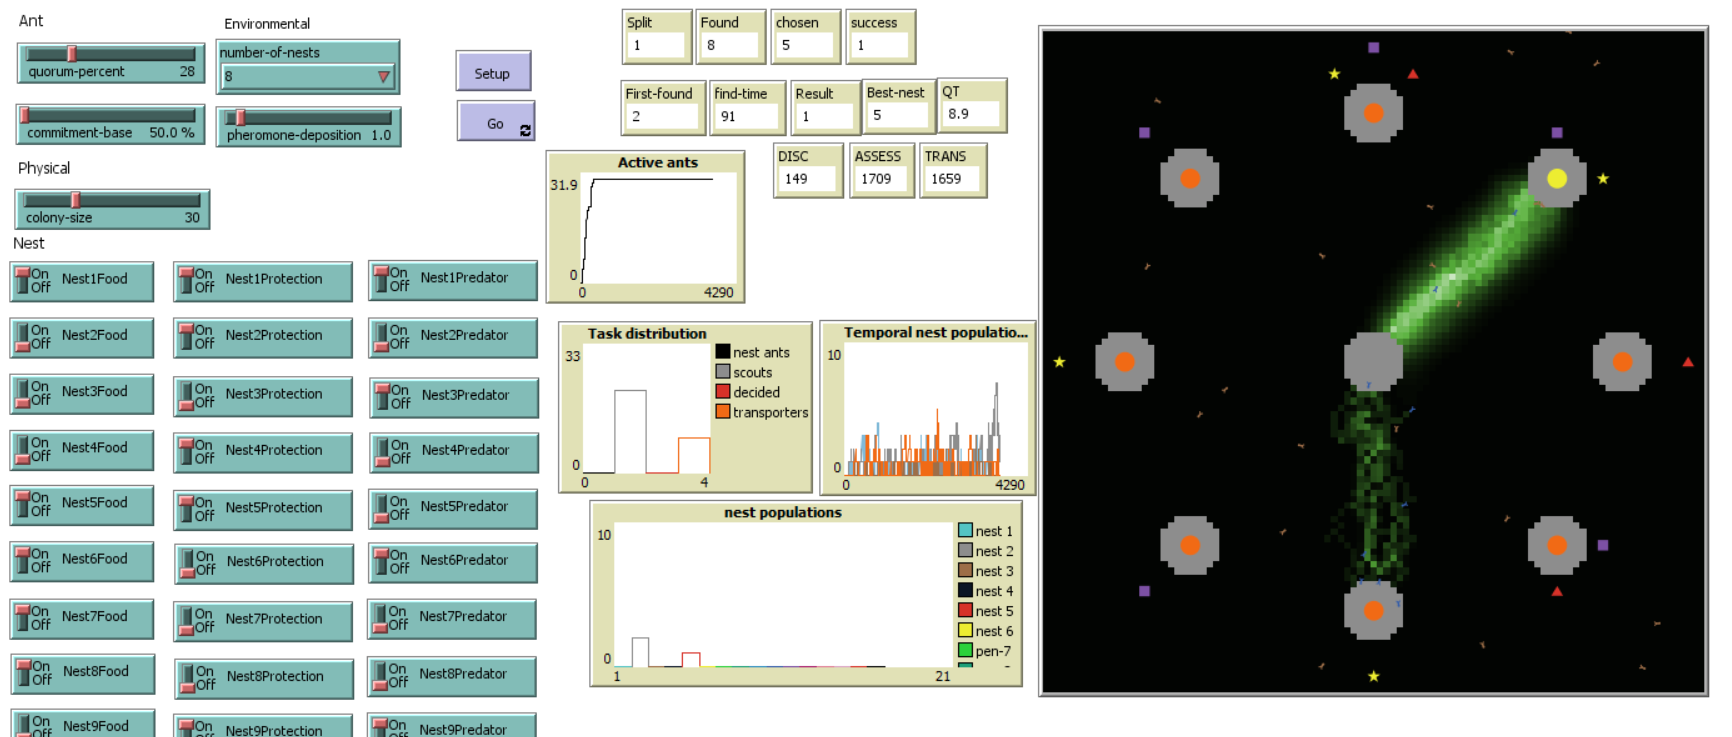
\includegraphics[width=.6\linewidth]{report-template/fig/netlogo.png}
	\caption{Model setup screenshot on NetLogo. On the left: the settings that the user can modify. In the middle: the obtained results. On the right: the real-time visualization of the simulation}
	\label{fig:netlogo}
\end{figure}

\subsection*{Implementation}
We distinguish 4 types of ants throughout the simulation :
\begin{itemize}
    \item Nest ants: Remain in the original nest until transitioning to become scout ants.
    \item Scout ants: Explore the area randomly or follow pheromone trails to evaluate the nests they find. When they discover a potential good nest, they become 'decided' ants.
    \item Decided ants: When an ant identifies a potential good nest, it goes back and forth between the original nest and the chosen nest. Each time it reaches the chosen nest, it checks whether the quorum has been reached. If this is the case, the ant becomes a transport ant; otherwise, it continues walking between the two nests. This type of ant can also revert to being a scout ant randomly, depending on the value of the parameter “commitment-base”.
    \item Transport ants: Move between the chosen and original nests, transporting brood until the relocation is complete.
\end{itemize}
To label a nest as “good” or “bad”, the ants have an internal threshold that they use as a comparison with the nest quality. In the initial model, when the ants only need to find a good nest, their threshold is a fixed value. However, in this model, where we want them to find the best nest possible (the one with the highest quality), their threshold is dynamically adjusted as they visit nests. Every time they encounter a nest with better quality than their current threshold, they update their threshold to match this quality. Conversely, when they find a nest with lower quality than their threshold, they label this nest as 'bad.' Over time, the only “good” nest left will be the best one (Figure \ref{fig:implementdiag}).

The ants' general behavior in this model is influenced by several parameters. We decided to focus on three specific parameters:
\subsubsection*{The quorum percent}, which represents the percentage of ants needed to visit a good nest for it to be chosen by the colony.
\subsubsection*{The commitment base} influences the probability of an ant reverting to being a scout after deciding on a nest.
\subsubsection*{Pheromone trails} are deposited by ants when moving, which aids navigation. An ant moves either randomly or follows these trails. We chose to study the influence of the quantity of pheromones deposited.\\

\begin{figure}
	\centering
	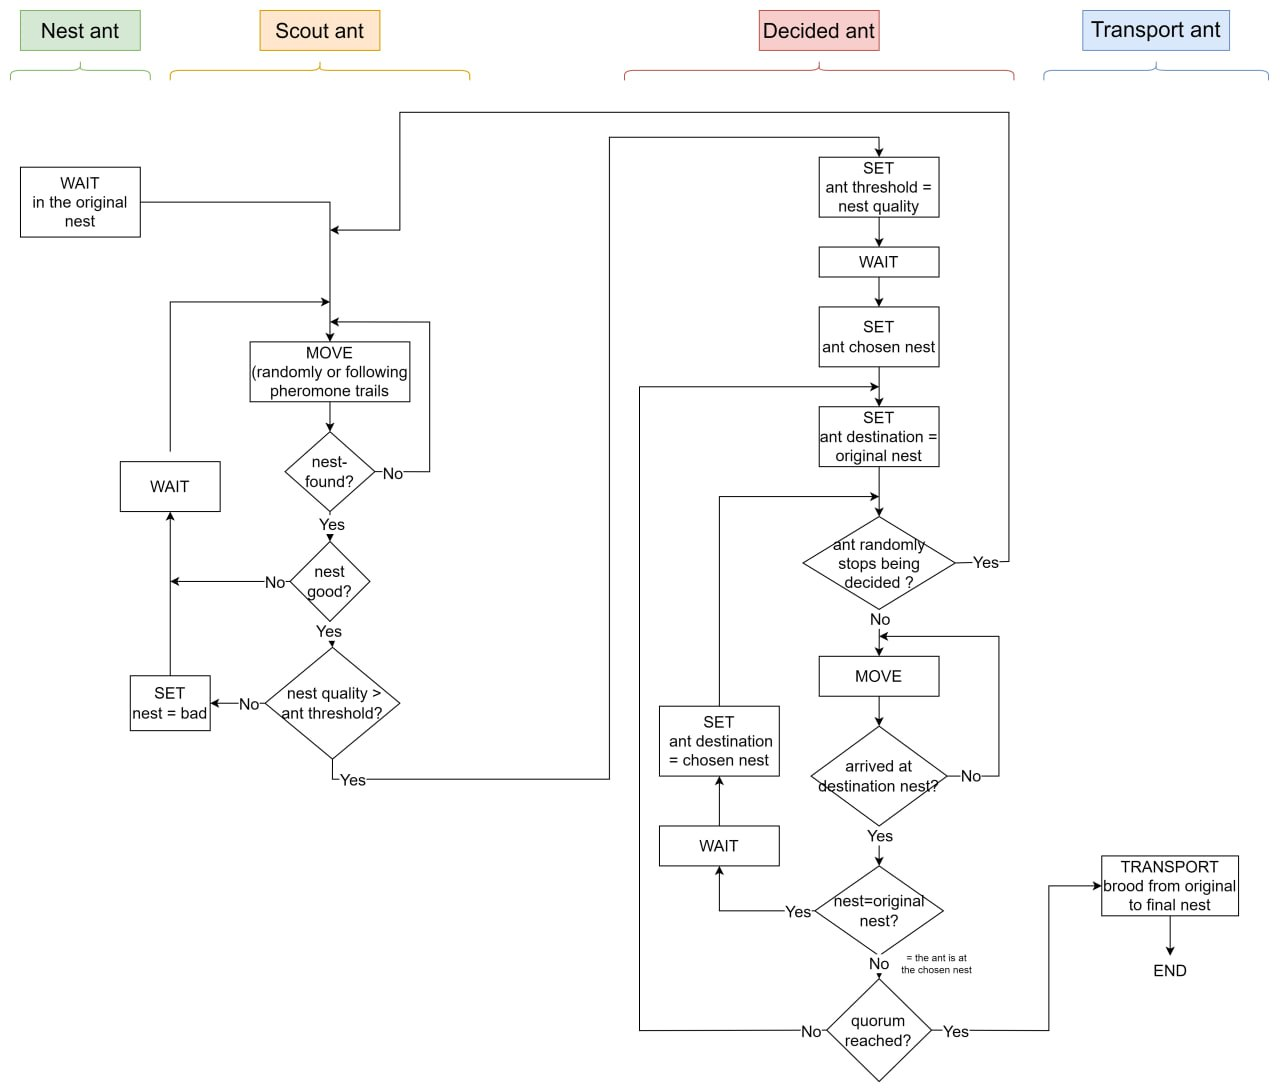
\includegraphics[width=.8\linewidth]{report-template/fig/implementation.jpeg}
	\caption{Simplified diagram of the model implementation algorithm}
	\label{fig:implementdiag}
\end{figure}
\section*{Tests and validation}
After implementing and verifying our code's functionality, we conducted multiple simulations to evaluate the model's performance in guiding ants toward the best nest under varying parameters. We specifically focused on three key parameters as stated before: quorum percentage, commitment-base percentage, and pheromone deposition. We tested different combinations of these parameters across various nest configurations, enabling us to assess ants' ability to find the best nest in diverse environments and study the impact of the specified parameters. During testing, we maintained a consistent setup with 30 ants, designated a single "best nest," and kept all other parameters at their default values outlined in the original paper.


\section*{Results}
From the different simulation setups we ran, we formed different conclusions according to the results we obtained. 

\subsubsection*{Ants overall decisions}
Depending on the environment setup, the ants were sometimes unable to find the best nest, regardless of the parameters. For example, when the number of nests was high, the ants struggled to choose the best one, often becoming "decided ants" before visiting all nests. Once decided, they failed to reassess nest quality, increasing the likelihood of the initially chosen nest being deemed the best. However, in simpler environments with fewer nests or nests of similar qualities nearby, they successfully chose the best one, contingent on the chosen parameters.

\subsubsection*{Quorum percent}
A high quorum rendered ants unable to choose a viable nest (resulting in no transporters) because more ants were required to validate a nest. Conversely, a too-low quorum led ants to quickly select the first good-quality nest without waiting to assess its potential as the best one. To optimize overall nest selection, we found the quorum should be set between 25\% and 50\%, depending on the complexity of the environment.

\subsubsection*{Commitment base}
This parameter exerted a significant influence: higher values resulted in poorer nest choices, as ants tended to select the first "good" nest without comparing it to others. Depending on the environment setup, this parameter should be set around 20-40\%.

\subsubsection*{Pheromone deposition}
While this parameter, specific to ants, influenced their movement and enabled them to check a nest's quorum, our observations indicated that it did not significantly impact simulation results.

\section*{Discussion}
To identify the best nest, ants compare them during the search phase when acting as scouts. However, once they commit to a nest, there is no reevaluation of its quality, following the behavior of the ants in the previous model. To enhance results, we propose modifying this behavior so that when another ant deems a nest as bad, decided ants on that nest revert to being scouts. This adjustment will be a focus in the upcoming phase, along with refining the parameters' influence. 

If time allows, we also plan to apply the model to another domain, specifically disaster response planning, where agents (such as drones) explore areas to determine optimal locations for establishing base camps, medical facilities, or supply distribution points during a disaster.\\\\

\section*{Conclusion}
In our study of ant colony behavior, we specifically enhanced the NetLogo model to emphasize the identification of the best nest during emigration, introducing parameters like food, protection, and predators with a unique focus on finding the best nest. Simulations, concentrating on quorum percentage, commitment base, and pheromone deposition, uncovered challenges in complex environments. Optimal quorum percentages (25\% to 50\%) and commitment base ranges (50-60\%) were identified, while pheromone deposition had minimal impact. Future work includes refining emigration behavior and testing the model in disaster response scenarios, building on our foundation for understanding collective decision-making in diverse environments. 

 
\acknow{ MC: tests and report; KG: setup, tests and report, BM: report; CS : setup, implementation, test and report.}
\showacknow % Display the acknowledgments section

% \pnasbreak splits and balances the columns before the references.
% If you see unexpected formatting errors, try commenting out this line
% as it can run into problems with floats and footnotes on the final page.
%\pnasbreak

\section*{\bibname}
\bibliographystyle{plain}
\bibliography{report-template/bib/bibliography}

\end{document}